\chapter{Calibrations in IQ-plane - Single Shot}
In this section the idea is, if one can calibrate some of the fundamental parts about our qubit by fitting distributions in the IQ-plane for readouts at different duration. We wait for the qubit to come to rest. Ideally in $\ket{0}$ but as the fridge is at non-zero temperature, we will also find a part of the population in $\ket{1}$. The experiment goes as follows.
\begin{itemize}
    \item Wait for equilibrium.
    \item For 50\% of the experiments apply an $X$-gate. Label the flipped qubits for $\ket{1}$ and the rest $\ket{0}$
    \item Measure for a set duration. This is done by applying a drive to the resonator at the dressed resonator frequency when the qubit is in state $\ket{0}$: $\omega_{drive} = \omega_r - \chi$
\end{itemize}
What we expect to see is that the qubit states of $\ket{1}$ will be pushed away. \footnote{This is beacuse we measure reflection/trasmission. We're free to perform displacement and rotations in the IQ plane since only magnitudes and phase \textbf{differences} have physical meaning.} 

\subsection{Theoretical Assumptions}
We now assume that the driving duration is so short that we will not see the qubits rotating back. Should not happen when driving in resonance with the one dressed frequency though. We will further assume, that a steady state is reached instantaneously. The state of the resonator in the IQ planer will then be constant unless the qubit decays/excites. 

We further assume that the characteristic decay times are much longer that the readout durations. This means: we can neglect the possibilities of decaying twice. For example $\ket{1} \to \ket{0} \to \ket{1}$ is prohibited in this simple model and we can assume that the decay process is linear.

These assumptions are a bit of a stretch but allow us a first analysis, where we only have to worry about doing a few linear fits.

\subsection{The Data}
The signal from the IQ plot is recorded in the digitizer and integrated up over the period. This experiment is done with a few different durations of measurement at $0.5, 1, 2, 5$ and $10 \mu s$. It is recorded wether an X-gate was applied before the measurement or not. An example of the data after $0.5 \mu s$ is given in Figure \ref{fig:raw_data_initial_IQ}.

\begin{figure}
    \centering
    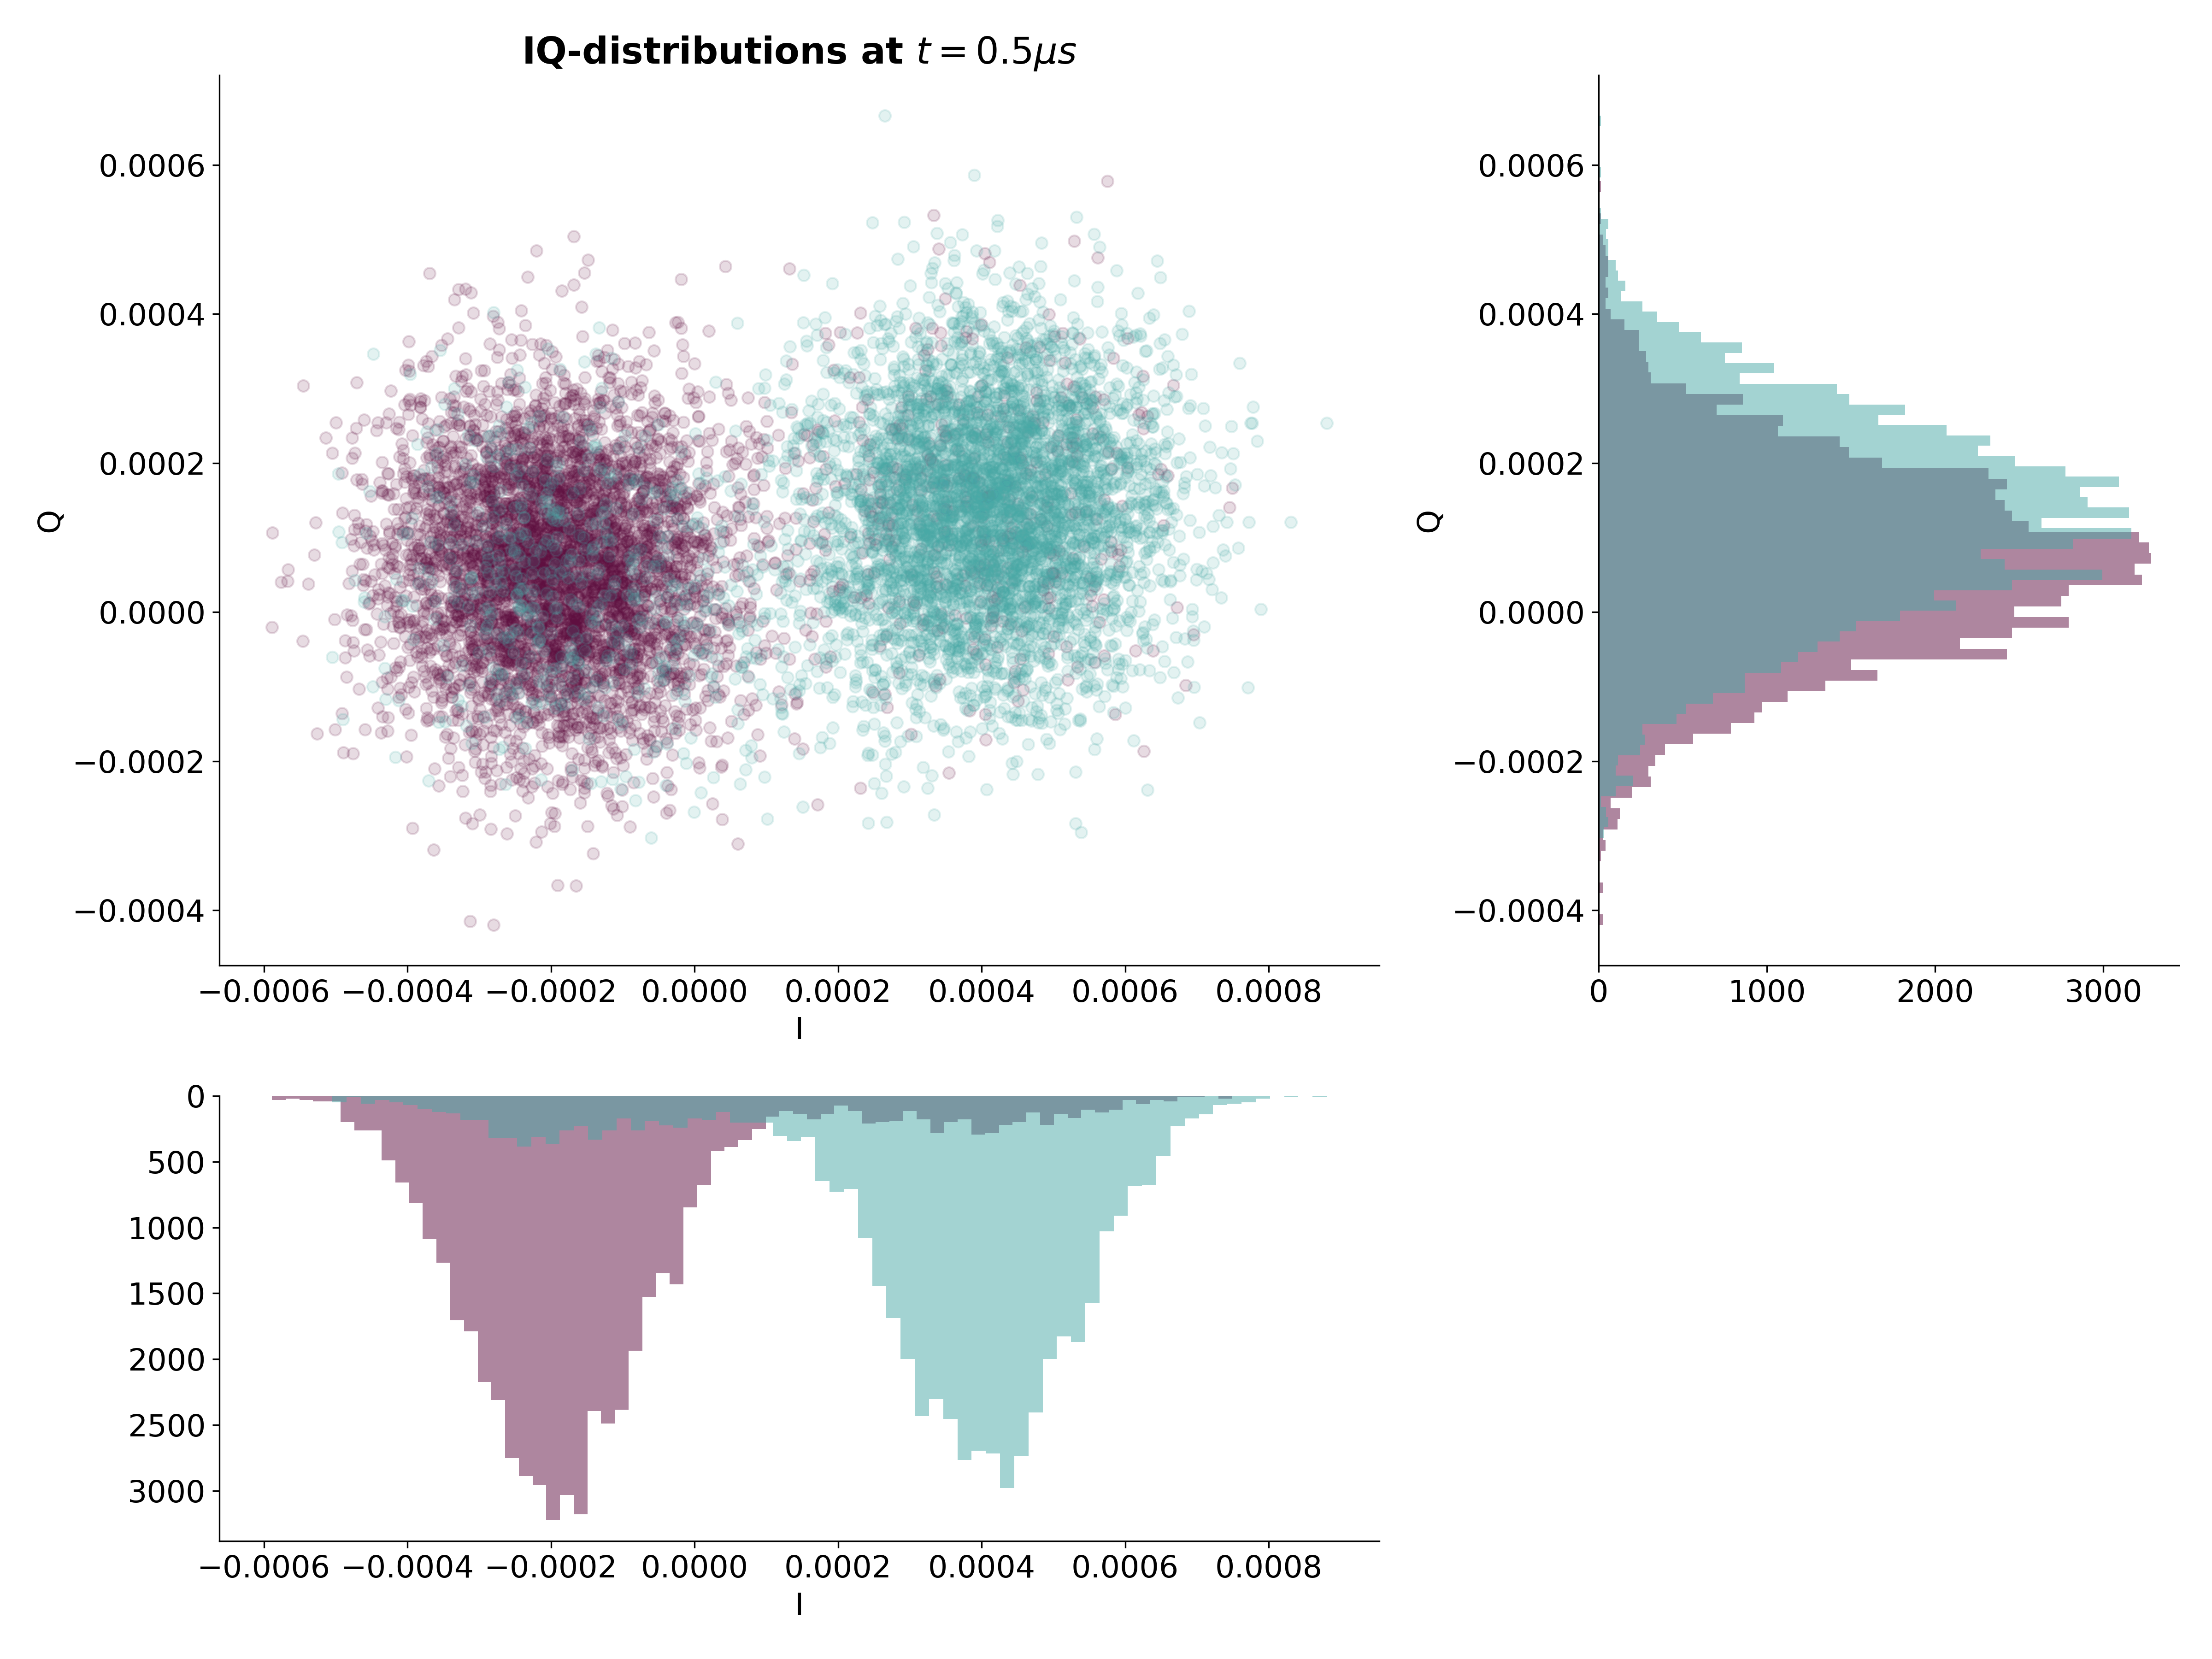
\includegraphics{Figs/Results/IQ_plane_initial/IQ_raw_at_0.5.png}
    \caption{The distributions from a heterodyne measurement of $0.5 \mu s$. The two distributions are from applying an X-gate or not, such that to the best of our knowledge the system is in state $\ket{0}$ or $\ket{1}$.}
    \label{fig:raw_data_initial_IQ}
\end{figure}


\subsection{Compounded Gauss with Uniform Mean}
For the T1 calibration, we need a distribution for the decayed state lying along the line between the two other distributions. Since every point comes with a Gaussian distribution around some mean, we will model this as a gaussian with a traveling mean.

As a first approach and to first order, where the growth in population is constant during the whole travel distance, we can take the mean to be uniformly taken from between the two Gaussians. We are given the mean for the two distributions: $\boldsymbol{\mu_1} = (\mu_{x1}, \mu_{y1})$ and $\boldsymbol{\mu_2} = (\mu_{x2}, \mu_{y2})$. To create a uniformly distribution between them, we will rotate and translate to place $\boldsymbol{\mu_1}$ in the origin and have $\boldsymbol{\mu_2}$ extend outwards along the x-direction. We perform the translation:
\begin{align*}
    x' = (x - \mu_{1x}) \hspace{1 cm} y' = y - \mu_{1y}
\end{align*}
and the rotation:
\begin{align*}
    \Tilde{x} = \cos\theta \; x' - \sin\theta \; y' \hspace{1cm} \Tilde{y} =  \sin\theta \; x' + \cos\theta \; y' 
\end{align*}
Where the angle is decided by:
\begin{equation}
    \tan \theta = - \frac{\mu_{y2}'}{\mu_{x2}'} 
\end{equation}
such that  $\boldsymbol{\mu_{2}}$ is on the x axis with $\Tilde{x} = |\boldsymbol{\mu_{2}} - \boldsymbol{\mu_{1}}|$.

In this new coordinate system, we have $\Tilde{\mu_{x2}}$ uniformly distributed from origin to $\mu_2$. If we now start with a 2d Gaussian in the new coordinates with $\sigma_x = \sigma_y = \sigma$, it will take the form:
\begin{equation}
    \frac{1}{2 \pi \sigma} \exp \left(- \frac{(\Tilde{x} - \Tilde{\mu_x})^2 + \Tilde{y^2}}{2 \; \sigma^2} \right)
\end{equation}
where the $\mu_y = 0$ in this frame. Now we have to take $\mu_x$ uniformly from the interval between $0$ and $r = |\boldsymbol{\mu_{2}} - \boldsymbol{\mu_{1}}|$. We get the following expression:

\begin{align}
    &\frac{1}{r} \int_0^r d\Tilde{\mu_x} \frac{1}{2 \pi \sigma^2} \exp \left(- \frac{(\Tilde{x} - \Tilde{\mu_x})^2 + \Tilde{y^2}}{2 \; \sigma^2} \right) \\
    = &\frac{1}{r}\frac{1}{\sqrt{2 \pi} \sigma} \Big(\erf((r + \Tilde{x}) / \sigma) - \erf(\Tilde{x} / \sigma)\Big) \exp(-\frac{\Tilde{y}^2}{2 \sigma^2})
\end{align}
Where the integration of $\Tilde{\mu_x}$ gives the error function, defined by: 
\begin{equation}
    \erf(x/\sigma) = \frac{1}{\sqrt{2 \pi }\sigma} \int_0^x dt e^{-t^2/2\sigma^2}
\end{equation}
This distribution can now be transferred back to the original coordinates. 

\subsection{Model}
To fit this data, we will split it in three parts:
\begin{enumerate}
    \item The main Gaussian distributions. This will be two-dimensional gaussian distribution with covariance $COV = \sigma^2 \cdot \identity$. Such that it has an even distribution in both the $I$ and $Q$ direction.
    \item The initilization error, which is modelled as a gaussian distribution with same covariance as the main one, but with a different mean. This mean is guessed (but for now not forced) to be in the center of the opposite distributions main Gaussian.
    \item The decay distribution. In the limits we opposed on the system, we can model the decays as a compound distribution of a gaussian with a uniform distribution of means between the main and the wrong-initilization-Gaussian. This model is desribed in the prior subsection. The standard deviation will still be the same as in the two above.  
\end{enumerate}
\noindent
Collecting these three parts, we have a distribution function with 7 parameters:

\begin{itemize}
    \item $\boldsymbol{\mu}_{\text{main}}$, $\boldsymbol{\mu}_{\text{wrong}}$ which are the two two-dimensional describing the center of the two gaussian distributions.
    \item $\sigma$ which is the standard deviation of all distributions.
    \item $f_{\text{wrong}},\; f_{\text{decay}}$ which are the fractions of the distribution in the wrong initialized state or in the decayed part. The fraction of the main gaussian is of course given as $f_{\text{main}} = 1 - f_{\text{wrong}} -f_{\text{decay}}$.
\end{itemize}

\noindent
And the total distribution is given as:

\begin{align}
    \PDF(I, Q) &= f_{\text{main}} \cdot \MVG\left[\boldsymbol{\mu}_{\text{main}}, \sigma^2\right](I, Q) \label{eq:pdf_of_iq_plane_distribution} \\
               &+ f_{\text{wrong}} \cdot \MVG\left[\boldsymbol{\mu}_{\text{wrong}}, \sigma^2\right](I, Q) \nonumber \\
               &+ f_{\text{decay}} \cdot \MVG\left[\Uniform\left[\boldsymbol{\mu}_{\text{main}}, \boldsymbol{\mu}_{\text{wrong}}\right], \sigma^2 \right](I, Q) \nonumber
\end{align}
where $\MVG\left[\boldsymbol{\mu}, \boldsymbol{\Sigma} \right]$ is a multivariate gaussian with mean $\boldsymbol{\mu}$ and covariance matrix $\boldsymbol{\Sigma}$, and $\Uniform{\boldsymbol{x, y}}$ is a uniform distribution of the points on the line between $\boldsymbol{x}$ and $\boldsymbol{y}$.

We now fit the data at $t = 0.5 \mu s$ which is seen from Figure \ref{fig:raw_data_initial_IQ} by using the Minuit Migrad minimizer to minimize the unbinned negative log likelihood function $\nLLH = \sum_i \log \PDF(I_i, Q_i)$, where the sum over $i$ refers to summing all data points. The results can be seen in Figure \ref{fig:fit_0_5_IQ_plane}.

\begin{figure*}
    \centering
    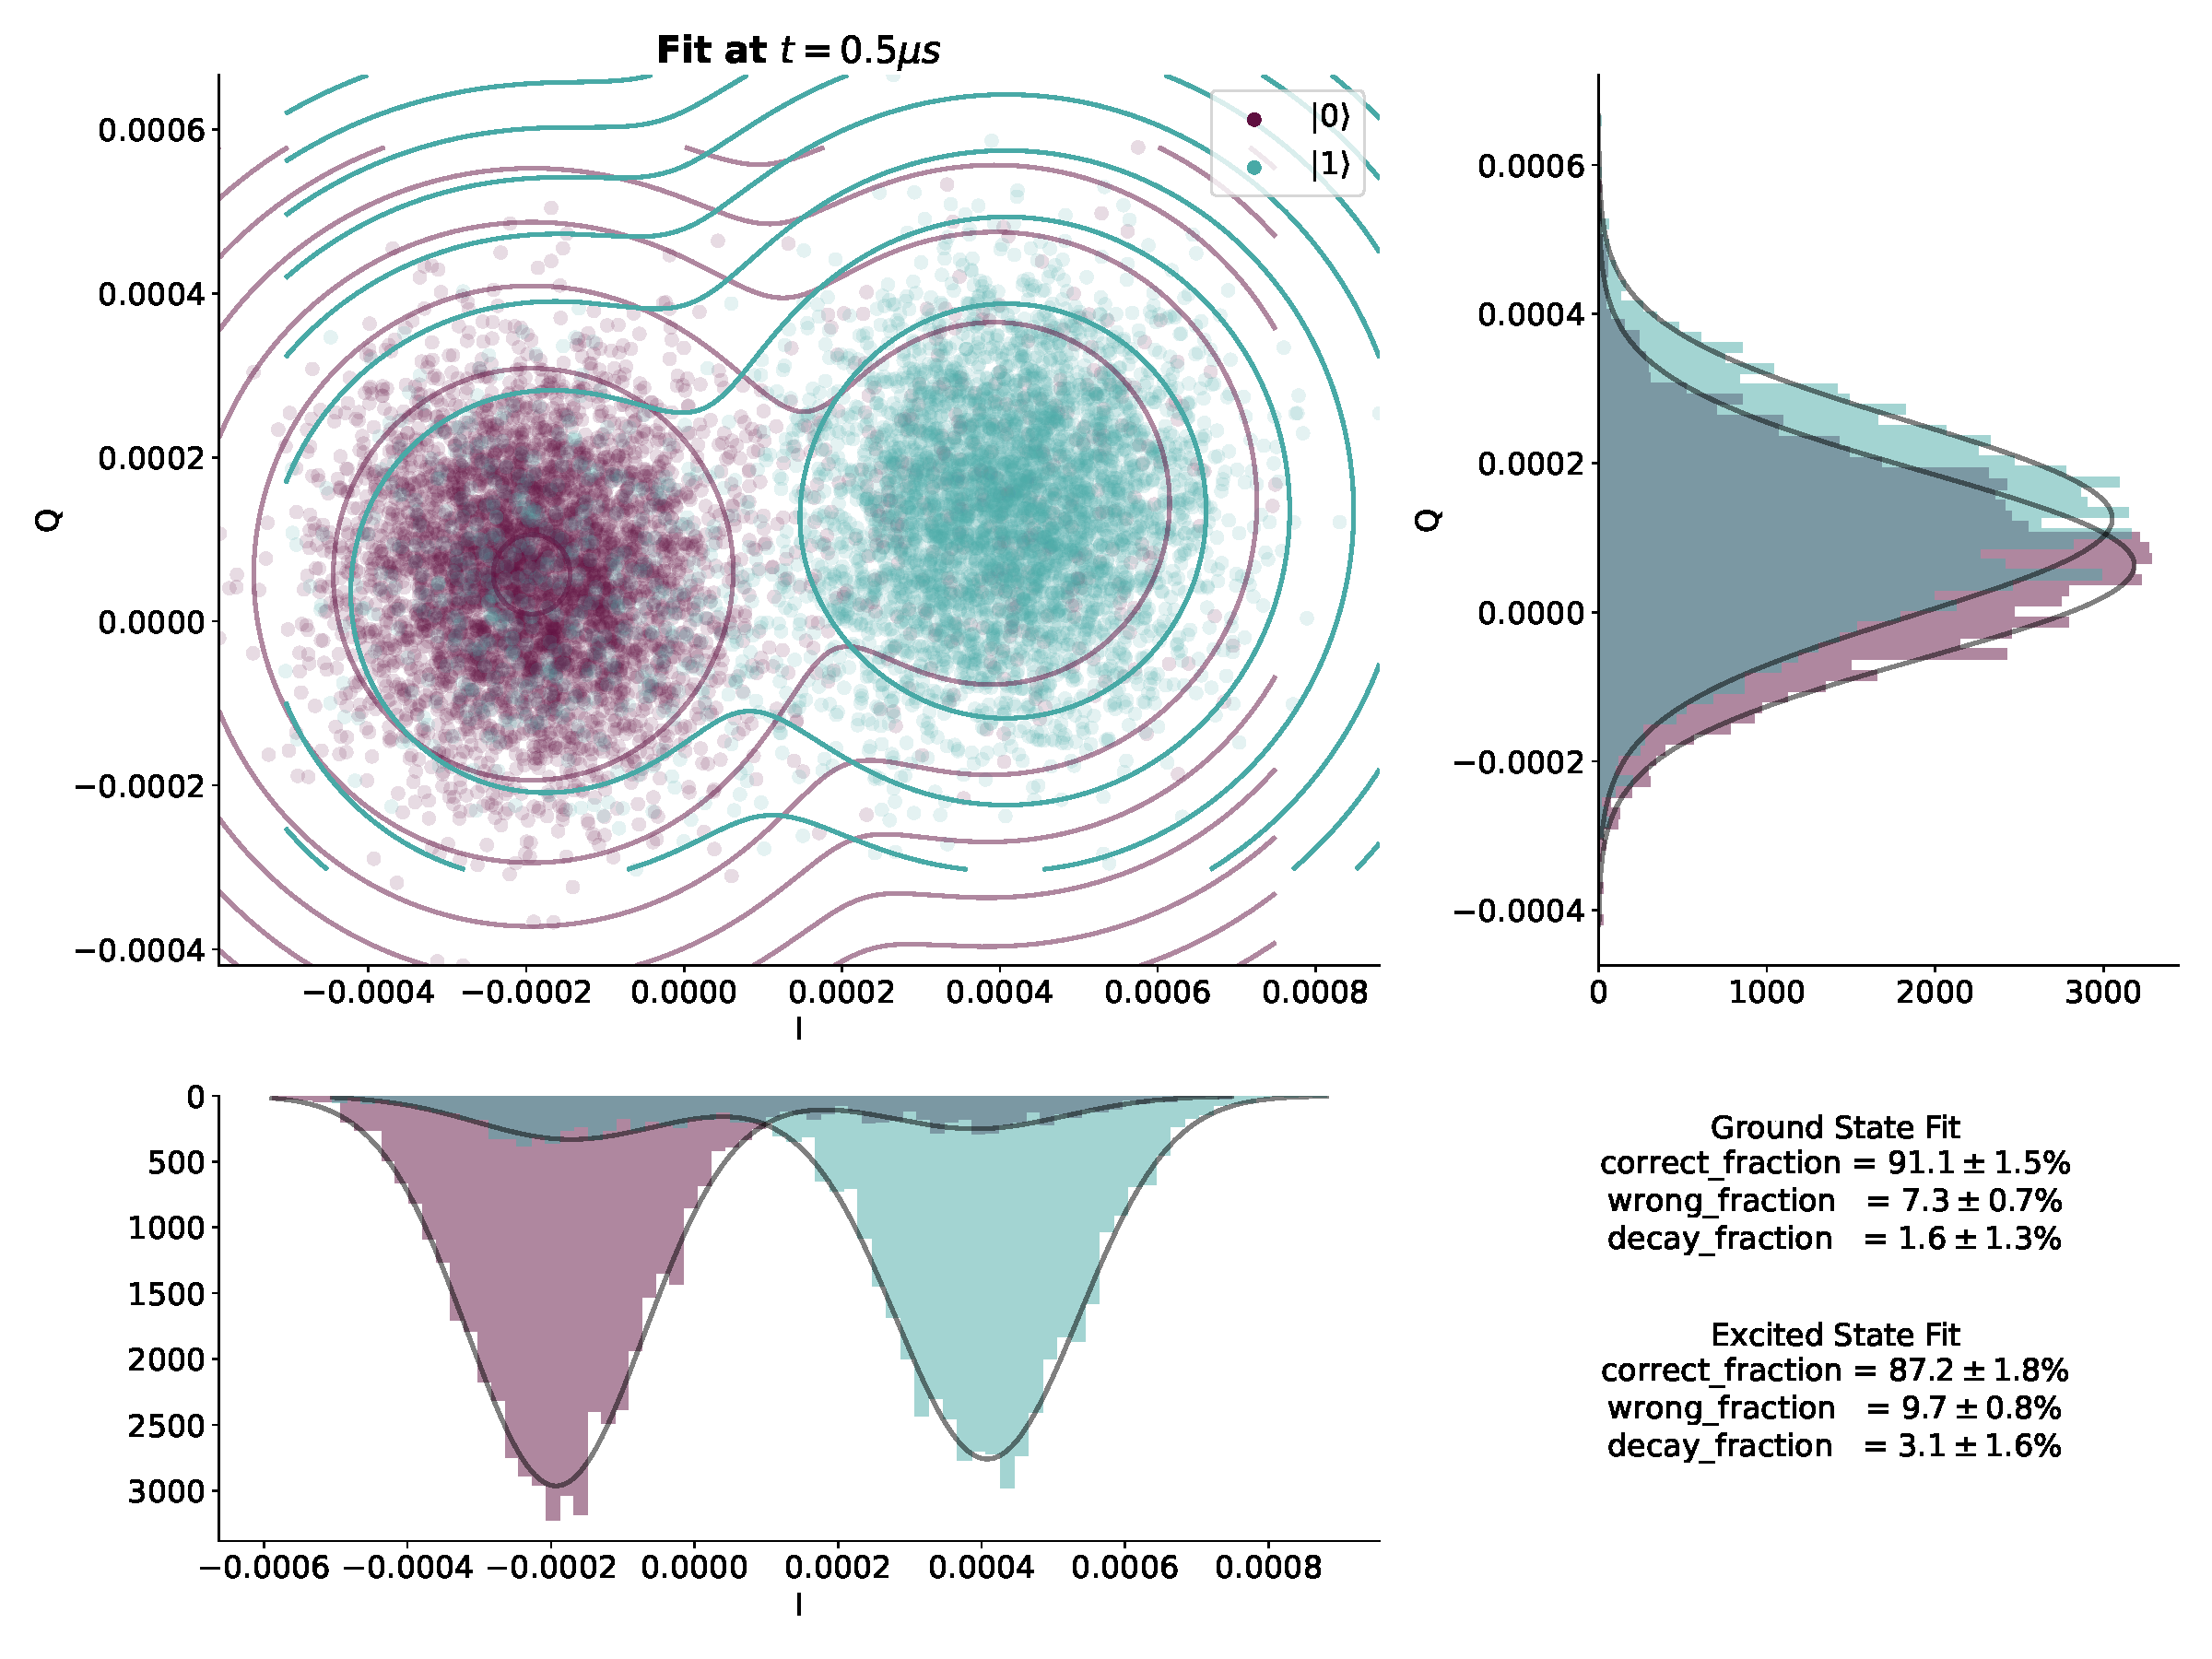
\includegraphics{Figs/Results/IQ_plane_initial/fit_0_5.pdf}
    \caption{The data from a $0.5 \mu s$ measurement fitted with the probability density distribution given in Equation \ref{eq:pdf_of_iq_plane_distribution}. The parameters from the fractions of distributions are given. The "wrong" and "decay" fractions are from the fit, and the correct fractions are error propagated from the two others. \textbf{While the other parameters could probably be found in the appendix.}}
    \label{fig:fit_0_5_IQ_plane}
\end{figure*}



\subsection{Evolution over Time}
Repeating the same fit procedure over the time for $t = 0.5, 1, 2, 5$ and $10 \; \mu s$, we can plot the fraction in each distribution as a function of time. This is done in Figure \ref{fig:evolution_of_fractions_in_fit}. Linear fits are also performed on the fitted fractional parameters and can be seen in \ref{tab:experimental_fit_parameters_IQ_plane}. The last $10 \; \mu s$ point is removed since it violates to many of our rough assumptions made earlier, and would not give us meaningful fit parameters.

\begin{figure}
    \centering
    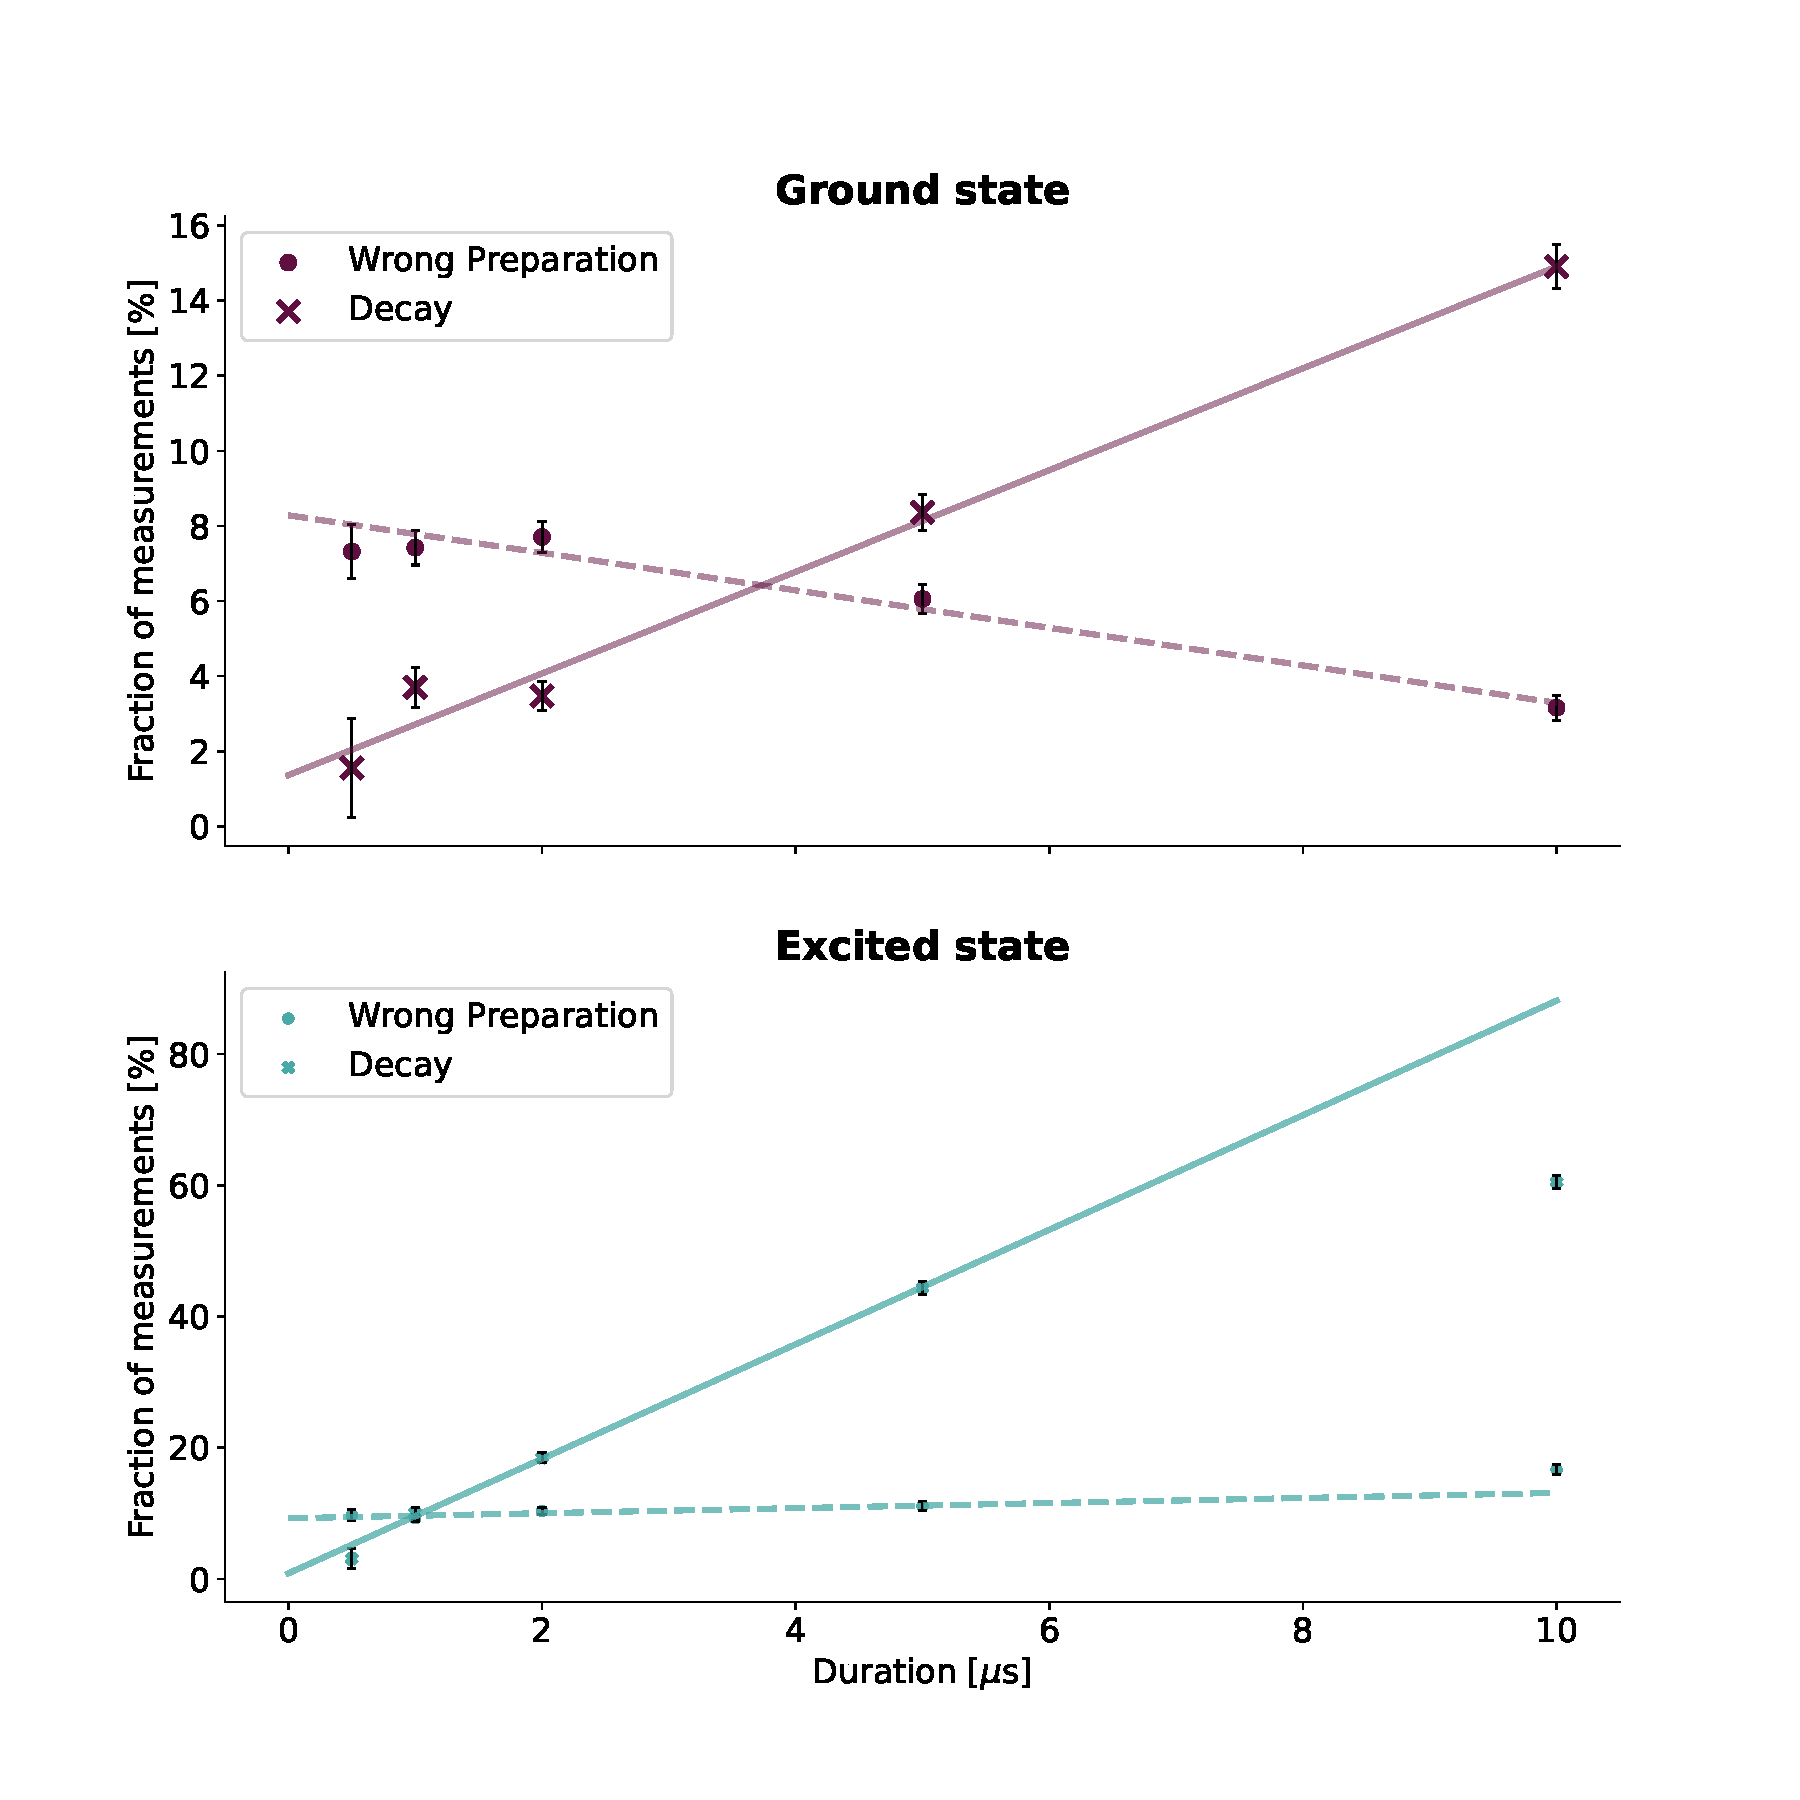
\includegraphics{Figs/Results/IQ_plane_initial/fraction_evolution.pdf}
    \caption[][2 cm]{Evolutioon the fitted parameters for $f_{\text{wrong}}$ and $f_{\text{decay}}$ for the two states $\ket{0}$ and $\ket{1}$ respectively. The linear fit paramters can be found in table \ref{tab:experimental_fit_parameters_IQ_plane}.}
    \label{fig:evolution_of_fractions_in_fit}
\end{figure}


\begin{table}
\centering
\begin{tabular}{l|c|c|c|c}
 & Initial Intercept & Initial Slope & $\chi^2$ & p-value \\
\hline
Ground Decay & $8.3 \pm 0.3 \%$ & $-0.5 \pm 0.1 \%$ & 3.3 & 0.353 \\
Ground Decay & $1.4 \pm 0.4 \%$ & $1.4 \pm 0.1 \%$ & 6.2 & 0.103 \\
Excited Decay & $9.2 \pm 0.5 \%$ & $0.4 \pm 0.2 \%$ & 0.9 & 0.634 \\
Excited Decay & $0.8 \pm 0.8 \%$ & $8.7 \pm 0.3 \%$ & 2.2 & 0.326 \\
\end{tabular}
\caption{Parameters and uncertainty from the linear fits of the fractions. }
\label{tab:experimental_fit_parameters_IQ_plane}
\end{table}


\subsection{Physical Parameters}
We use the above approach to do some calibration. The following parameters are possible to find:
\begin{itemize}
\item $T_{1\uparrow}$ - decay time
\item $T_{1\downarrow}$ - excitation time 
\item The equilibrium distribution $\ket{0}$
\item The x-gate fidelity 
\item The temperature should be found from both comparing the rate of excitation/decay and from the equilibrium distribution.
\end{itemize}

The actual distributions for these will be that the distribution will follow $(1 - e^{-t/T_1})$, or to first order $(t/T_1)$, which is what we have used in this fits. This is of course an approximation to low order in $t/T_1$. We correlate the slope to $T_1$ by $1 / \Gamma$, where $\Gamma$ is the slope/decay rate of the fit.
We find:
\begin{itemize}
    \item Excited state decay time: T1-down: 11.45 +- 0.38 us
    \item Ground  state decay time: T1-up: 73.82 +- 0.10 us
    \item Gamma: 	 0.101 +/- 0.003 / us
    \item T1: 	 9.915 +/- 0.297 us
    \item X gate infidelty: 	 1.0 +- 0.6 %
\end{itemize}

\paragraph{Temperature}
We now have two ways to find the temperature. The first is to use the equilibrium distribution and the second is to use the decay rate.

In equilibrium, the relation between the $p_1/p_0 = \tanh(-\beta \hbar \omega / 2)$, where $\omega$ is the energy difference between the two states.

We have the same relation between the two decay rates: $\Gamma_{1\uparrow} / \Gamma_{1\downarrow} = \exp(-\beta \hbar \omega)$

Temperature: 	 127.9 +/- 2.9 mK

Temperature: 	 153.6 +/- 5.4 mK
